\documentclass[10pt]{beamer}

\usetheme[progressbar=frametitle]{metropolis}
\usepackage{appendixnumberbeamer}

\usepackage{booktabs}
\usepackage[scale=2]{ccicons}
\usepackage{listings}
% % \usetheme[progressbar=frametitle]{metropolis}
\usepackage{appendixnumberbeamer}
\usepackage[utf8]{vietnam}
\usepackage[utf8]{inputenc}
\usepackage[vietnamese]{babel}
\usepackage[T1]{fontenc}
%\renewcommand\sfdefault{cmbr}
\usepackage{booktabs}
\usepackage[scale=2]{ccicons}
\usepackage{ragged2e}
\apptocmd{\frame}{}{\justifying}{}
\usepackage{pgfplots}
\usepgfplotslibrary{dateplot}
\usepackage[upright]{fourier}
\usepackage{tikz}



\usetikzlibrary{matrix,arrows,decorations.pathmorphing}


\definecolor{rosy}{RGB}{247, 215, 148}
\definecolor{summer}{RGB}{245, 205, 121}
\definecolor{beige}{RGB}{253, 227, 167}
\definecolor{sblack}{RGB}{64, 64, 64}
\setbeamercolor{frametitle}{bg=rosy,%bg=beige,
fg=sblack}

\usepackage{hyperref}
\hypersetup{
    colorlinks=true,
    linktoc=all,
    linkcolor=black,
}
\usepackage{relsize}
\usepackage{textpos}
\addtobeamertemplate{frametitle}{}{%
\begin{textblock*}{100mm}(\textwidth,-1.05cm)
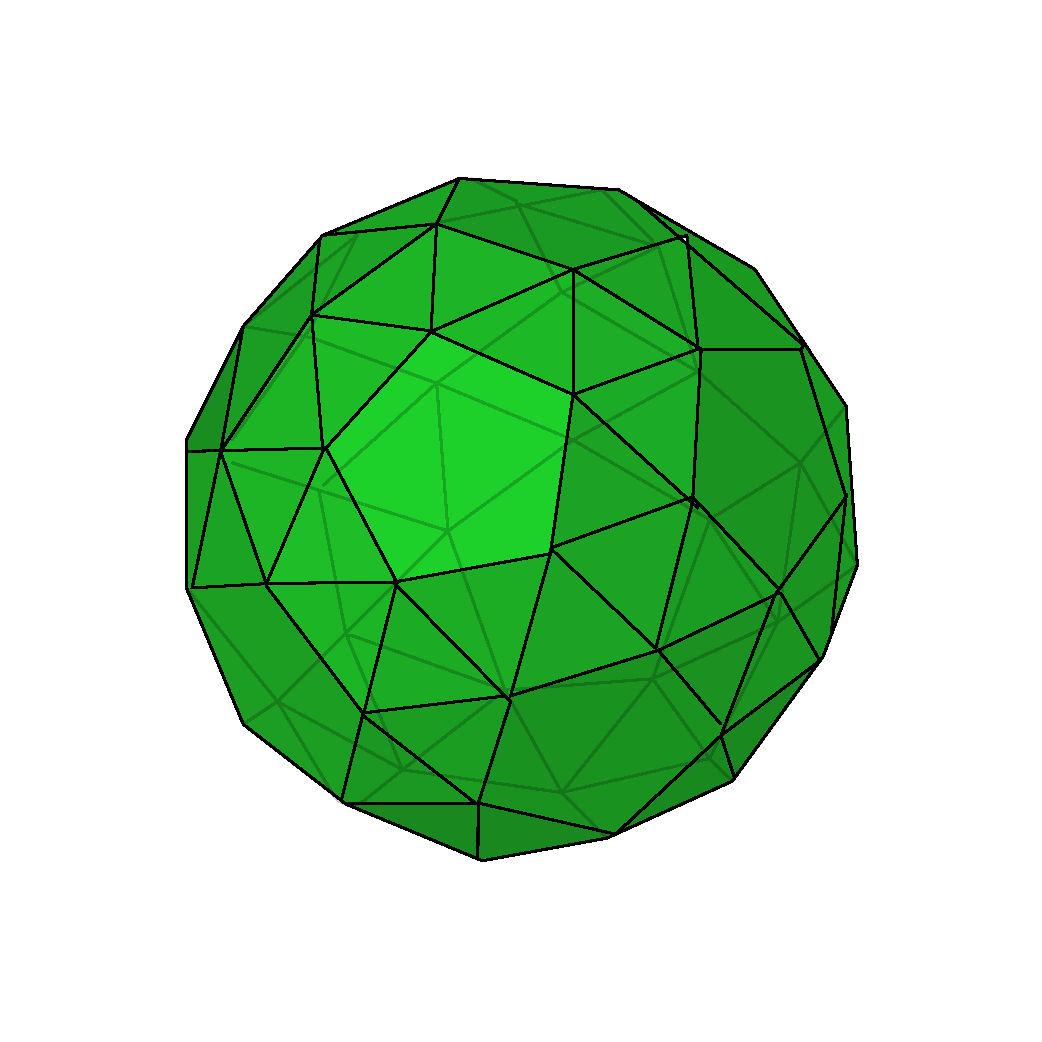
\includegraphics[height=1cm,width=1cm,keepaspectratio]{logo.pdf}
\end{textblock*}}

\usepackage{xspace}

\setbeamerfont{page number in head/foot}{size=\tiny}
\setbeamercolor{footline}{fg=gray}
\setbeamertemplate{frame footer}{PiMA 2019: The Mathematics of Deep Learning}

% \newcommand{\themename}{\textbf{\textsc{metropolis}}\xspace}
\usepackage{cmbright}

\usepackage{pgfplots}
\usepgfplotslibrary{dateplot}

\usepackage{xspace}
\newcommand{\themename}{\textbf{\textsc{metropolis}}\xspace}

\title{LẬP TRÌNH PYTHON}
\subtitle{PiMA 2019 - Python cơ bản}
\date{\today}
\date{}
\author{Phan Ngọc Tiên}
\institute{York University, Toronto, Canada}
%\titlegraphic{\hfill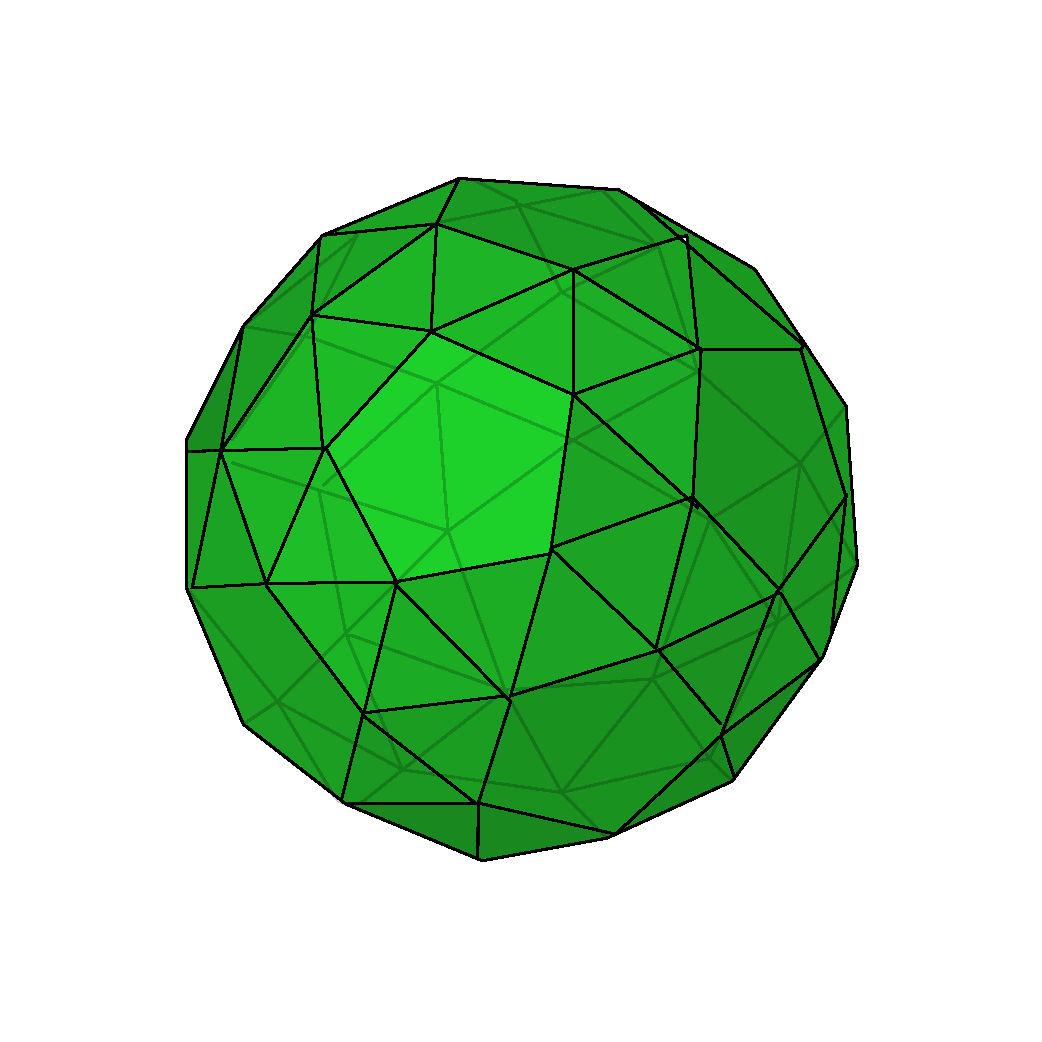
\includegraphics[height=1.5cm]{logo.pdf}}

\begin{document}

\maketitle

\begin{frame}{Mục lục}
  \setbeamertemplate{section in toc}[sections numbered]
  \tableofcontents[hideallsubsections]
\end{frame}

\section{Giới thiệu về Python}
\begin{frame}{Giới thiệu về Python}
  \begin{itemize}
    \item Python là ngôn ngữ lập trình bậc cao, ra mắt lần đầu vào năm 1991
    \item Python là ngôn ngữ lập trình đơn giản, cú pháp (syntax) đơn giản, dễ  đọc, rất gần với ngôn ngữ tự nhiên
    \item Hỗ trợ lập trình hướng cấu trúc, lập trình hướng cấu trúc và lập trình hàm (yếu)
  \end{itemize}
\end{frame}

\begin{frame}[fragile]{Basic Input/Output (Nhập xuất cơ bản)}
  \begin{verbatim}
    # Input (Nhập)
    x = input()

    # Output (Xuất)
    print(x)
  \end{verbatim}
\end{frame}

\begin{frame}[fragile]{Các phép toán}
  \begin{itemize}
    \item Python hỗ trợ các phép toán $+, -, *, /$ (chia lấy kết quả float), $//$ (chia lấy phần nguyên, kết quả int), $**$ (lên lũy thừa).

    \item Các phép biến đổi bit: $\&$ (AND), $|$ (OR), $\ \^$ (XOR).

    \item Đối với biến logic có \textbf{and, or, not}.

    \item Các phép toán so sánh $<$ (nhỏ hơn), $>$ (lớn hơn), $<=$ (nhỏ hơn hoặc bằng), $>=$ (lớn hơn hoặc bằng), $==$ (bằng)

  \end{itemize}
\end{frame}

\begin{frame}[fragile]{Các kiểu dữ liệu}
  \begin{itemize}
    \item Python tạo kiểu động (dynamically typed)
  \end{itemize}
  \begin{columns}
    \begin{column}{0.4\textwidth}
      \begin{verbatim}
        # Số nguyên (Integer)
        x = 20
        # Số thực (Float)
        y = 17.5
        # Số phức (Complex)
        z = 20 + 17j
      \end{verbatim}
    \end{column}
    \begin{column}{0.7\textwidth}
      \begin{verbatim}
        #include <iostream>
        #include <complex>
        using namespace std;

        int main() {
        int x = 20;
        double y = 17.5;
        complex<double> z4 = 1.5 + 2i;
        }
      \end{verbatim}
    \end{column}
  \end{columns}
\end{frame}

\begin{frame}[fragile]{Các kiểu dữ liệu: Boolean}
  \begin{columns}
    \begin{column}{0.4\textwidth}
      \begin{verbatim}
        # Boolean
        x = True
        y = False
      \end{verbatim}
    \end{column}
    \begin{column}{0.7\textwidth}
      \begin{verbatim}
        #include <iostream>
        #include <complex>
        using namespace std;

        int main() {
        bool x = true;
        bool y = false;
        }
      \end{verbatim}
    \end{column}
  \end{columns}
\end{frame}

\begin{frame}[fragile]{Các kiểu dữ liệu: String (Chuỗi)}
  \begin{itemize}
    \item Python
    \begin{verbatim}
      # String (Chuỗi)
      x = "PiMA 2019 'Deep Learning'"
    \end{verbatim}

    \item C++
    \begin{verbatim}
      #include <iostream>
      #include <string>
      using namespace std;

      int main() {
      string s = "PiMA 2019 'Deep Learning'";
      }
    \end{verbatim}
  \end{itemize}

\end{frame}


\begin{frame}[fragile]{Các kiểu dữ liệu: List (Danh sách)}

  \begin{itemize}
    \item Python
    \begin{verbatim}
      x = [1, 2, 3, 4, 5]
      # List can be nested (danh sách có thể lồng vào nhau)
      x = [[1, 2, 3], [4, 5, 6]]

      ## Có thể có nhiều kiểu dữ liệu trong cùng 1 danh sách
      x = [[3.14, 2], 3 + 4j, [5, 6]]
    \end{verbatim}
    \item C++
    \begin{verbatim}
      #include <iostream>
      #include <vector>
      using namespace std;
      int main() {
      int arr[] = {1, 2, 3, 4, 5, 6};
      vector <double> a {3.14, 2.71, 2.11};
      }
    \end{verbatim}
  \end{itemize}
\end{frame}

\begin{frame}[fragile]{Các kiểu dữ liệu: Dictionary (Từ Điển)}
  \begin{verbatim}
    x = {"P": "Project",
    "i": "in",
    "M": "Mathematics",
    "A": "Applications"}
  \end{verbatim}
\end{frame}

\begin{frame}[fragile]{Các kiểu dữ liệu: Tuple}
  \begin{verbatim}
    point = (1, 2, 3)

    # Lấy ra giá trị từ tuple
    x, y, z = point
  \end{verbatim}


  \only<2>{\Large Tuple vs List: điểm giống và khác nhau giữa List và Tuple là gì?}
\end{frame}


\begin{frame}[fragile]{Python cơ bản}
  Refer to notebook.
\end{frame}

\begin{frame}[fragile]{Hàm (function)}

\end{frame}

\section{Titleformats}

\begin{frame}{Metropolis titleformats}
  \themename supports 4 different titleformats:
  \begin{itemize}
    \item Regular
    \item \textsc{Smallcaps}
    \item \textsc{allsmallcaps}
    \item ALLCAPS
  \end{itemize}
  They can either be set at once for every title type or individually.
\end{frame}

{
\metroset{titleformat frame=smallcaps}
\begin{frame}{Small caps}
  This frame uses the \texttt{smallcaps} titleformat.

  \begin{alertblock}{Potential Problems}
    Be aware, that not every font supports small caps. If for example you typeset your presentation with pdfTeX and the Computer Modern Sans Serif font, every text in smallcaps will be typeset with the Computer Modern Serif font instead.
  \end{alertblock}
\end{frame}
}

{
\metroset{titleformat frame=allsmallcaps}
\begin{frame}{All small caps}
  This frame uses the \texttt{allsmallcaps} titleformat.

  \begin{alertblock}{Potential problems}
    As this titleformat also uses smallcaps you face the same problems as with the \texttt{smallcaps} titleformat. Additionally this format can cause some other problems. Please refer to the documentation if you consider using it.

    As a rule of thumb: Just use it for plaintext-only titles.
  \end{alertblock}
\end{frame}
}

{
\metroset{titleformat frame=allcaps}
\begin{frame}{All caps}
  This frame uses the \texttt{allcaps} titleformat.

  \begin{alertblock}{Potential Problems}
    This titleformat is not as problematic as the \texttt{allsmallcaps} format, but basically suffers from the same deficiencies. So please have a look at the documentation if you want to use it.
  \end{alertblock}
\end{frame}
}

\section{Elements}

\begin{frame}[fragile]{Typography}
  \begin{verbatim}The theme provides sensible defaults to
    \emph{emphasize} text, \alert{accent} parts
    or show \textbf{bold} results.\end{verbatim}

    \begin{center}becomes\end{center}

      The theme provides sensible defaults to \emph{emphasize} text,
      \alert{accent} parts or show \textbf{bold} results.
    \end{frame}

    \begin{frame}{Font feature test}
      \begin{itemize}
        \item Regular
        \item \textit{Italic}
        \item \textsc{SmallCaps}
        \item \textbf{Bold}
        \item \textbf{\textit{Bold Italic}}
        \item \textbf{\textsc{Bold SmallCaps}}
        \item \texttt{Monospace}
        \item \texttt{\textit{Monospace Italic}}
        \item \texttt{\textbf{Monospace Bold}}
        \item \texttt{\textbf{\textit{Monospace Bold Italic}}}
      \end{itemize}
    \end{frame}

    \begin{frame}{Lists}
      \begin{columns}[T,onlytextwidth]
        \column{0.33\textwidth}
        Items
        \begin{itemize}
          \item Milk \item Eggs \item Potatos
        \end{itemize}

        \column{0.33\textwidth}
        Enumerations
        \begin{enumerate}
          \item First, \item Second and \item Last.
        \end{enumerate}

        \column{0.33\textwidth}
        Descriptions
        \begin{description}
          \item[PowerPoint] Meeh. \item[Beamer] Yeeeha.
        \end{description}
      \end{columns}
    \end{frame}
    \begin{frame}{Animation}
      \begin{itemize}[<+- | alert@+>]
        \item \alert<4>{This is\only<4>{ really} important}
        \item Now this
        \item And now this
      \end{itemize}
    \end{frame}
    \begin{frame}{Figures}
      \begin{figure}
        \newcounter{density}
        \setcounter{density}{20}
        \begin{tikzpicture}
          \def\couleur{alerted text.fg}
          \path[coordinate] (0,0)  coordinate(A)
          ++( 90:5cm) coordinate(B)
          ++(0:5cm) coordinate(C)
          ++(-90:5cm) coordinate(D);
          \draw[fill=\couleur!\thedensity] (A) -- (B) -- (C) --(D) -- cycle;
          \foreach \x in {1,...,40}{%
          \pgfmathsetcounter{density}{\thedensity+20}
          \setcounter{density}{\thedensity}
          \path[coordinate] coordinate(X) at (A){};
          \path[coordinate] (A) -- (B) coordinate[pos=.10](A)
          -- (C) coordinate[pos=.10](B)
          -- (D) coordinate[pos=.10](C)
          -- (X) coordinate[pos=.10](D);
          \draw[fill=\couleur!\thedensity] (A)--(B)--(C)-- (D) -- cycle;
          }
        \end{tikzpicture}
        \caption{Rotated square from
        \href{http://www.texample.net/tikz/examples/rotated-polygons/}{texample.net}.}
      \end{figure}
    \end{frame}
    \begin{frame}{Tables}
      \begin{table}
        \caption{Largest cities in the world (source: Wikipedia)}
        \begin{tabular}{lr}
          \toprule
          City & Population\\
          \midrule
          Mexico City & 20,116,842\\
          Shanghai & 19,210,000\\
          Peking & 15,796,450\\
          Istanbul & 14,160,467\\
          \bottomrule
        \end{tabular}
      \end{table}
    \end{frame}
    \begin{frame}{Blocks}
      Three different block environments are pre-defined and may be styled with an
      optional background color.

      \begin{columns}[T,onlytextwidth]
        \column{0.5\textwidth}
        \begin{block}{Default}
          Block content.
        \end{block}

        \begin{alertblock}{Alert}
          Block content.
        \end{alertblock}

        \begin{exampleblock}{Example}
          Block content.
        \end{exampleblock}

        \column{0.5\textwidth}

        \metroset{block=fill}

        \begin{block}{Default}
          Block content.
        \end{block}

        \begin{alertblock}{Alert}
          Block content.
        \end{alertblock}

        \begin{exampleblock}{Example}
          Block content.
        \end{exampleblock}

      \end{columns}
    \end{frame}
    \begin{frame}{Math}
      \begin{equation*}
        e = \lim_{n\to \infty} \left(1 + \frac{1}{n}\right)^n
      \end{equation*}
    \end{frame}
    \begin{frame}{Line plots}
      \begin{figure}
        \begin{tikzpicture}
          \begin{axis}[
            mlineplot,
            width=0.9\textwidth,
            height=6cm,
            ]

            \addplot {sin(deg(x))};
            \addplot+[samples=100] {sin(deg(2*x))};

          \end{axis}
        \end{tikzpicture}
      \end{figure}
    \end{frame}
    \begin{frame}{Bar charts}
      \begin{figure}
        \begin{tikzpicture}
          \begin{axis}[
            mbarplot,
            xlabel={Foo},
            ylabel={Bar},
            width=0.9\textwidth,
            height=6cm,
            ]

            \addplot plot coordinates {(1, 20) (2, 25) (3, 22.4) (4, 12.4)};
            \addplot plot coordinates {(1, 18) (2, 24) (3, 23.5) (4, 13.2)};
            \addplot plot coordinates {(1, 10) (2, 19) (3, 25) (4, 15.2)};

            \legend{lorem, ipsum, dolor}

          \end{axis}
        \end{tikzpicture}
      \end{figure}
    \end{frame}
    \begin{frame}{Quotes}
      \begin{quote}
        Veni, Vidi, Vici
      \end{quote}
    \end{frame}

    {%
    \setbeamertemplate{frame footer}{My custom footer}
    \begin{frame}[fragile]{Frame footer}
      \themename defines a custom beamer template to add a text to the footer. It can be set via
      \begin{verbatim}\setbeamertemplate{frame footer}{My custom footer}\end{verbatim}
      \end{frame}
      }

      \begin{frame}{References}
        Some references to showcase [allowframebreaks] \cite{knuth92,ConcreteMath,Simpson,Er01,greenwade93}
      \end{frame}

      \section{Conclusion}

      \begin{frame}{Summary}

        Get the source of this theme and the demo presentation from

        \begin{center}\url{github.com/matze/mtheme}\end{center}

          The theme \emph{itself} is licensed under a
          \href{http://creativecommons.org/licenses/by-sa/4.0/}{Creative Commons
          Attribution-ShareAlike 4.0 International License}.

          \begin{center}\ccbysa\end{center}

          \end{frame}

          {\setbeamercolor{palette primary}{fg=black, bg=yellow}
          \begin{frame}[standout]
            Questions?
          \end{frame}
          }

          \appendix

          \begin{frame}[fragile]{Backup slides}
            Sometimes, it is useful to add slides at the end of your presentation to
            refer to during audience questions.

            The best way to do this is to include the \verb|appendixnumberbeamer|
            package in your preamble and call \verb|\appendix| before your backup slides.

            \themename will automatically turn off slide numbering and progress bars for
            slides in the appendix.
          \end{frame}

          \begin{frame}[allowframebreaks]{References}

            \bibliography{demo}
            \bibliographystyle{abbrv}

          \end{frame}

          \end{document}
